%%%%%%%%%%%%%%%%%%%%%%%%%%%%%%%%%%%%%%%%%
% Beamer Presentation
% LaTeX Template
% Version 1.0 (10/11/12)
%
% This template has been downloaded from:
% http://www.LaTeXTemplates.com
%
% License:
% CC BY-NC-SA 3.0 (http://creativecommons.org/licenses/by-nc-sa/3.0/)
%
%%%%%%%%%%%%%%%%%%%%%%%%%%%%%%%%%%%%%%%%%

%----------------------------------------------------------------------------------------
%	PACKAGES AND THEMES
%----------------------------------------------------------------------------------------

\documentclass{beamer}

\mode<presentation> {
	
	% The Beamer class comes with a number of default slide themes
	% which change the colors and layouts of slides. Below this is a list
	% of all the themes, uncomment each in turn to see what they look like.
	
	%\usetheme{default}
	%\usetheme{AnnArbor}
	%\usetheme{Antibes}
	%\usetheme{Bergen}
	%\usetheme{Berkeley}
	%\usetheme{Berlin}
	%\usetheme{Boadilla}
	%\usetheme{CambridgeUS}
	%\usetheme{Copenhagen}
	%\usetheme{Darmstadt}
	%\usetheme{Dresden}
	%\usetheme{Frankfurt}
	%\usetheme{Goettingen}
	%\usetheme{Hannover}
	%\usetheme{Ilmenau}
	%\usetheme{JuanLesPins}
	%\usetheme{Luebeck}
	\usetheme{Madrid}
	%\usetheme{Malmoe}
	%\usetheme{Marburg}
	%\usetheme{Montpellier}
	%\usetheme{PaloAlto}
	%\usetheme{Pittsburgh}
	%\usetheme{Rochester}
	%\usetheme{Singapore}
	%\usetheme{Szeged}
	%\usetheme{Warsaw}
	
	% As well as themes, the Beamer class has a number of color themes
	% for any slide theme. Uncomment each of these in turn to see how it
	% changes the colors of your current slide theme.
	
	%\usecolortheme{albatross}
	\usecolortheme{beaver}
	%\usecolortheme{beetle}
	%\usecolortheme{crane}
	%\usecolortheme{dolphin}
	%\usecolortheme{dove}
	%\usecolortheme{fly}
	%\usecolortheme{lily}
	%\usecolortheme{orchid}
	%\usecolortheme{rose}
	%\usecolortheme{seagull}
	%\usecolortheme{seahorse}
	%\usecolortheme{whale}
	%\usecolortheme{wolverine}
	
	%\setbeamertemplate{footline} % To remove the footer line in all slides uncomment this line
	%\setbeamertemplate{footline}[page number] % To replace the footer line in all slides with a simple slide count uncomment this line
	
	%\setbeamertemplate{navigation symbols}{} % To remove the navigation symbols from the bottom of all slides uncomment this line
}

\usepackage{graphicx} % Allows including images
\usepackage{subfigure}
\usepackage{booktabs} % Allows the use of \toprule, \midrule and \bottomrule in tables
\usepackage{bm}

%----------------------------------------------------------------------------------------
%	TITLE PAGE
%----------------------------------------------------------------------------------------

\title[CPCA inference]{Asymptotic Theory for Common Principla Component Analysis} 

\author{Ganchao Wei} 
\date{October 13, 2021}

\begin{document}
	
	\begin{frame}
		\titlepage % Print the title page as the first slide
	\end{frame}
	
	\begin{frame}
		\frametitle{Overview} % Table of contents slide, comment this block out to remove it
		\tableofcontents
	\end{frame}
	
	%--------------------------------------------------------------------
	%	PRESENTATION SLIDES
	%--------------------------------------------------------------------
	
	\section{Introduction}
	
	\begin{frame}
		\frametitle{Introduction}
		\textbf{Common principle component analysis (CPCA)}: the $p\times p$ covariance matrices of $k$ populations can be diagonalized by the same orthogonal transformation.\\
		\textbf{Thehypothesis of common principal components (CPC's)}.  $\bm{H}_C: \bm{\beta}'\bm{\Sigma}_i\bm{\beta}= \bm{\Lambda}_i$, for $i=1,\ldots,k$\\
		We can further arrange $\bm{\beta}$ according to the first group, i.e. $\bm{\beta}'_1\bm{\Sigma}_1\bm{\beta}_1 > \bm{\beta}'_2\bm{\Sigma}_1\bm{\beta}_2 > \ldots > \bm{\beta}'_p\bm{\Sigma}_1\bm{\beta}_p$\\
		
		\textbf{Notations \& Assumptions}:
		\begin{itemize}
			\item 
			$\bm{\Sigma}_i$ are p.d.s.
			\item
			$\bm{\Lambda}_i = diag(\lambda_{i1},\ldots,\lambda_{ip})$
			\item
			$n_i\bm{S}_i \sim W_p(n_i, \Sigma_i)$
			\item
			The ML estimates are $\hat{\bm{\beta}} = (\hat{\bm{\beta}}_1,\ldots, \hat{\bm{\beta}}_p)$ and $\hat{\bm{\Lambda}}_i = diag(\hat{\lambda}_{i1},\ldots,\hat{\lambda}_{ip})$
		\end{itemize}
	\end{frame}

	\section{Asymptotic distribution of MLE}

%----------------------------------------------
\begin{frame}
	\frametitle{Asymptotic distribution of MLE}
	The log-likelihood function of the $k$ samples, up to an additive constant:
	\begin{figure}
		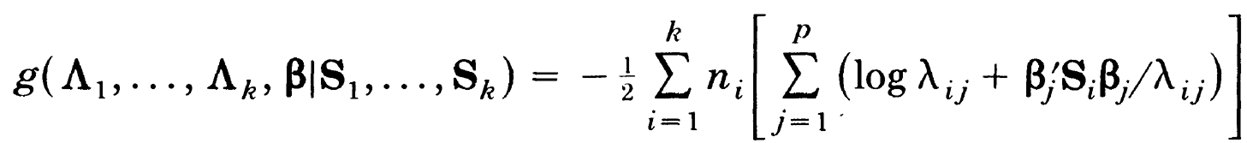
\includegraphics[width=0.8\linewidth]{image001.png}
	\end{figure}
Let $\lambda_{(i)}' = (\lambda_{i1},\ldots,\lambda_{ip})$, $n = n_1+\ldots+n_k$ and $r_i = n_i/n$. Then the information matrix is:
\begin{figure}
	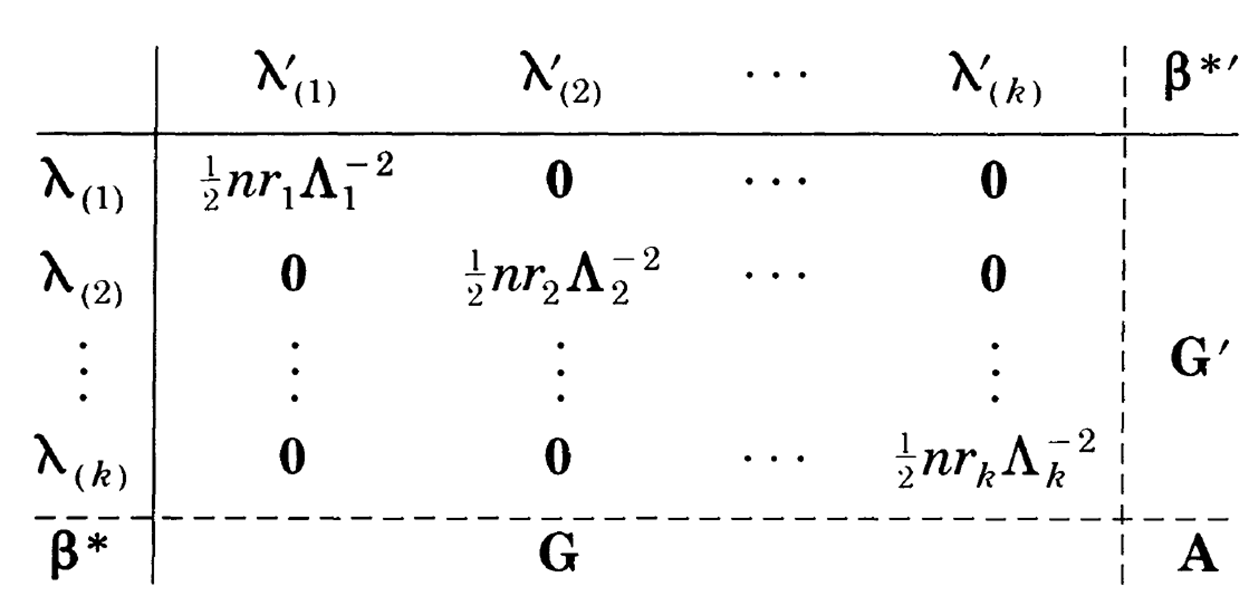
\includegraphics[width=0.6\linewidth]{image002.png}
\end{figure}	
	, where $\bm{G}$ and $\bm{A}$ are not yet determined.
\end{frame}

%----------------------------------------------
\begin{frame}
	\frametitle{Asymptotic distribution of MLE (eigenvalues)}
	Use the asymptotic normality of $n_i\bm{S}_i$ to get the asymptotic univariate distribution of $\hat{\lambda}_{ij}$ as
	$$\sqrt{n_i}(\hat{\lambda}_{ij} - \lambda_{ij}) \sim N(0, 2\lambda_{ij}^2)$$
	From the Fisher information, the joint asymptotic distribution of $(\hat{\lambda}'_{(1)},\ldots,\hat{\lambda}'_{(k)})'$ has covariance matrix
	\begin{figure}
		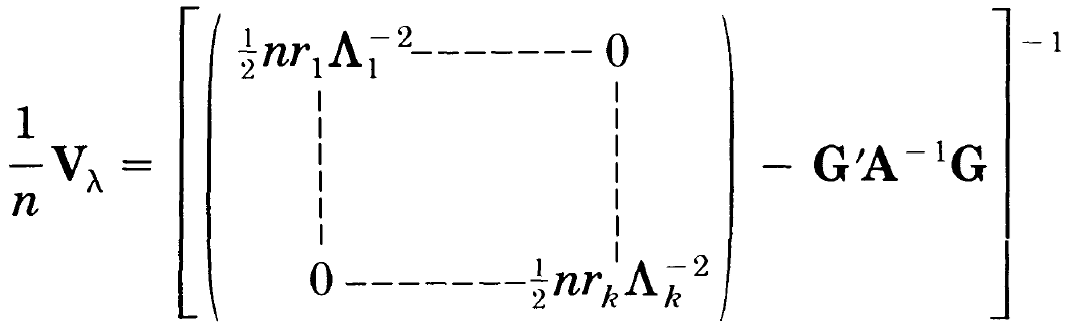
\includegraphics[width=0.6\linewidth]{image003.png}
	\end{figure}
By comparison, we can see that $\bm{G} = \bm{0}$. Therefore,
	\begin{figure}
	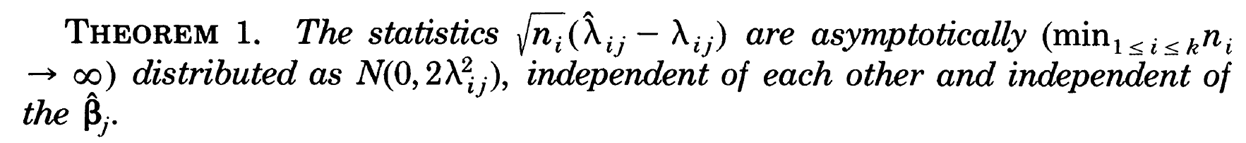
\includegraphics[width=0.9\linewidth]{image004.png}
\end{figure} 
\end{frame}
	

%----------------------------------------------
\begin{frame}
	\frametitle{Asymptotic distribution of MLE (eigenvectors)}
	Let $\bm{V}_i$ be the asymptotic covariance matrix of $\sqrt{n_i}vec(\hat{\bm{\beta}}) = \sqrt{n}(\hat{\bm{\beta}}'_1,\ldots,\hat{\bm{\beta}}'_k)'$. Further, define:
	\begin{figure}
		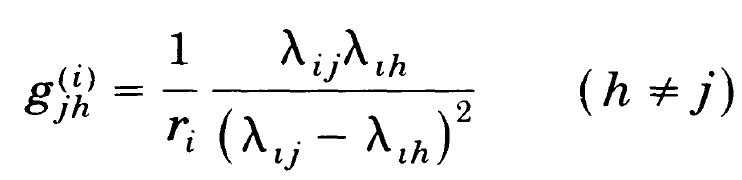
\includegraphics[width=0.4\linewidth]{image005.png}
	\end{figure}
	Then, we get
	\begin{figure}
		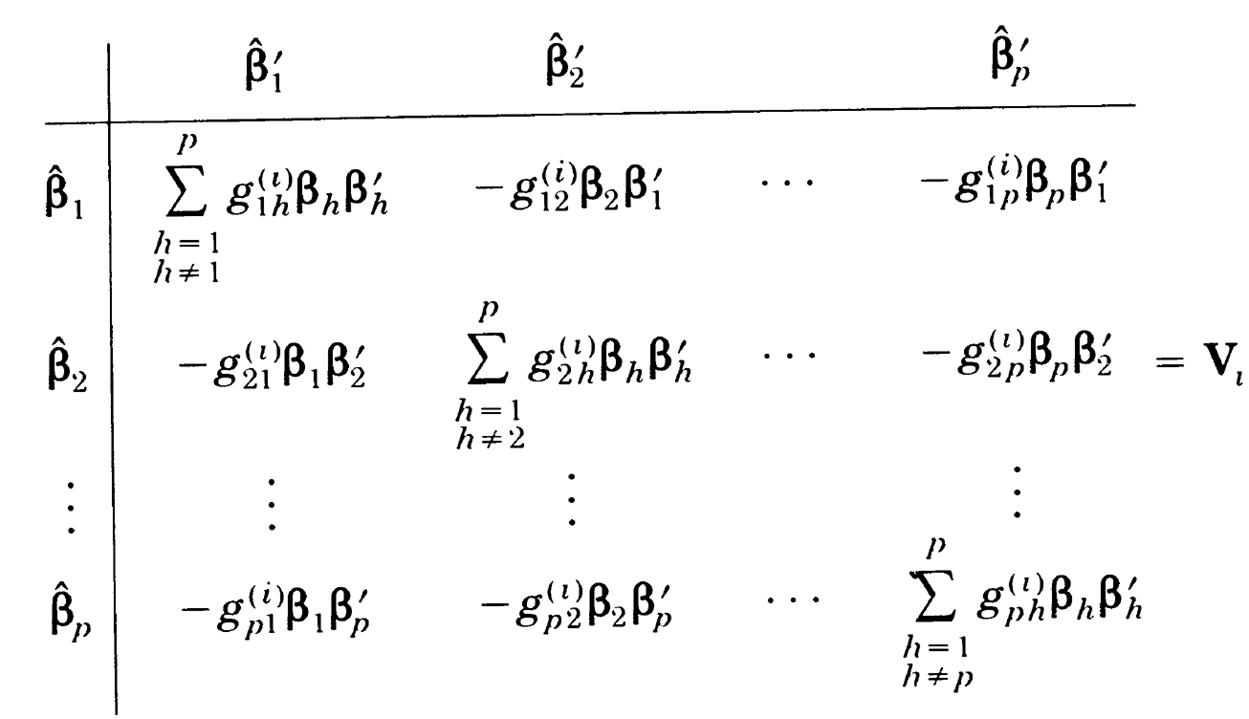
\includegraphics[width=0.7\linewidth]{image006.png}
	\end{figure}
\end{frame}


%----------------------------------------------
\begin{frame}
	\frametitle{Asymptotic distribution of MLE (eigenvectors)}
	Since $\bm{V}_i$ are simultaneously diagonalizable, there exists an orthogonal matrix $\bm{H}$, s.t.
	\begin{figure}
		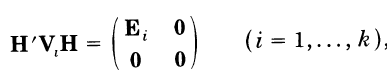
\includegraphics[width=0.5\linewidth]{image007.png}
	\end{figure}
Then we can get the information matrix for the transformed variable $\bm{u} = \bm{H}'_1 vec \hat{\bm{\beta}}$ as
\begin{figure}
	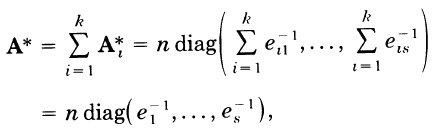
\includegraphics[width=0.5\linewidth]{image008.png}
\end{figure}
\end{frame}

%----------------------------------------------
\begin{frame}
	\frametitle{Asymptotic distribution of MLE (eigenvectors)}
	Then transform back and write out $\bm{H}_1$ explicitly, we can get
	\begin{figure}
		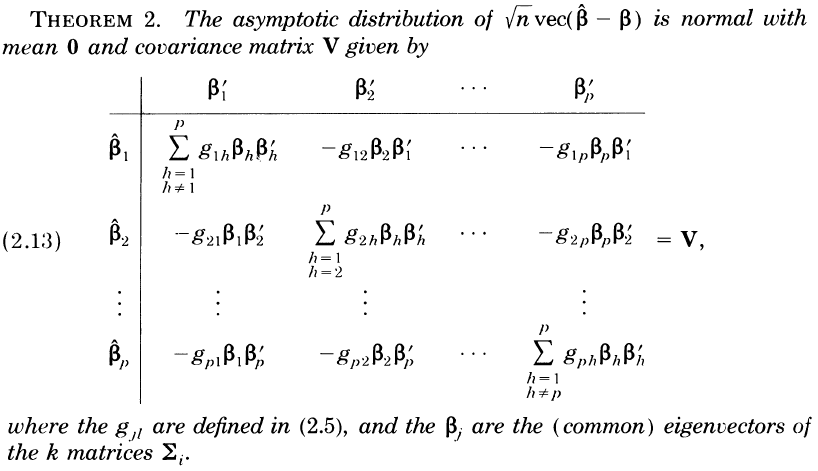
\includegraphics[width=0.9\linewidth]{image009.png}
	\end{figure}
\end{frame}

\section{test for q hypothetical eigenvectors}


%----------------------------------------------
\begin{frame}
	\frametitle{An asymptotic test for q hypothetical eigenvectors}
	The null hypothesis is $H_q: (\bm{\beta}_1,\ldots,\bm{\beta}_q) = (\bm{\beta}_1^0,\ldots,\bm{\beta}_q^0)$, which is based on the submatrix of asymptotic covariance $\bm{V}$. Denote the submatrix as $\bm{V}(q)$. $\bm{V}(q)$ has following eigenstructure:
	\begin{figure}
		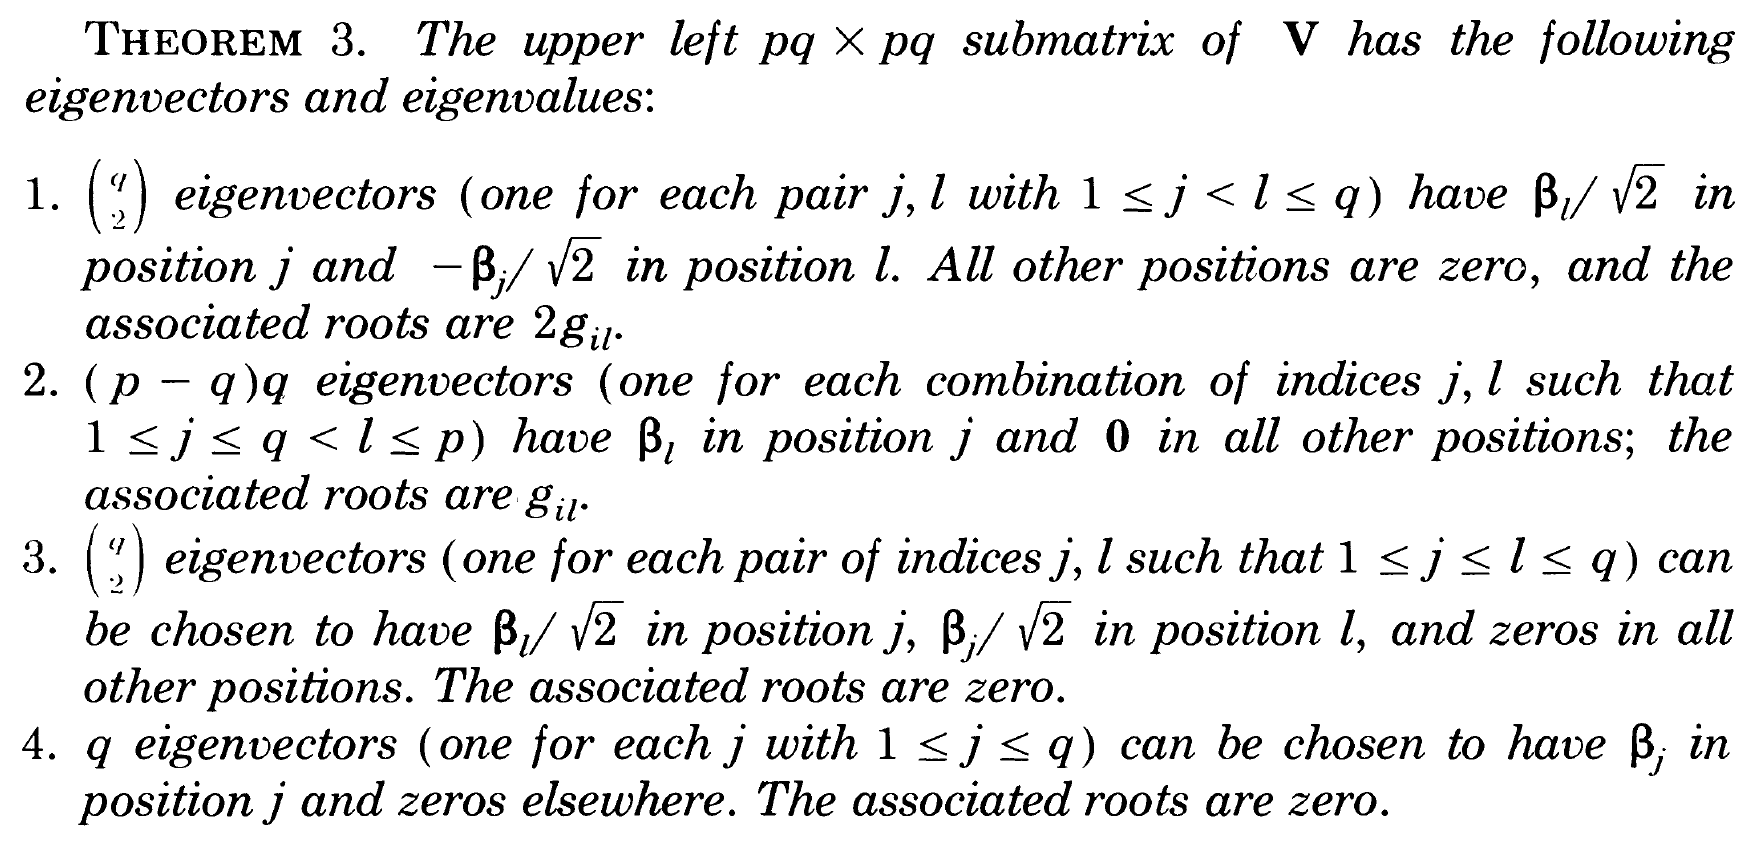
\includegraphics[width=0.9\linewidth]{image010.png}
	\end{figure}
\end{frame}

%----------------------------------------------
\begin{frame}
	\frametitle{An asymptotic test for q hypothetical eigenvectors}
	Let $\bm{\Phi} $ be a diagonal matrix with diagonal elements equal to the nonzero roots of $\bm{V}(q)$, i.e. $\bm{\Phi} = diag(2g_{12},\ldots,2g_{q-1,1},g_{1,q+1},\ldots,g_{qp})$. Also let the columns of matrix $\Gamma$ be given by the characteristic vectors associated with the nonzero roots. Then, 
	\begin{figure}
		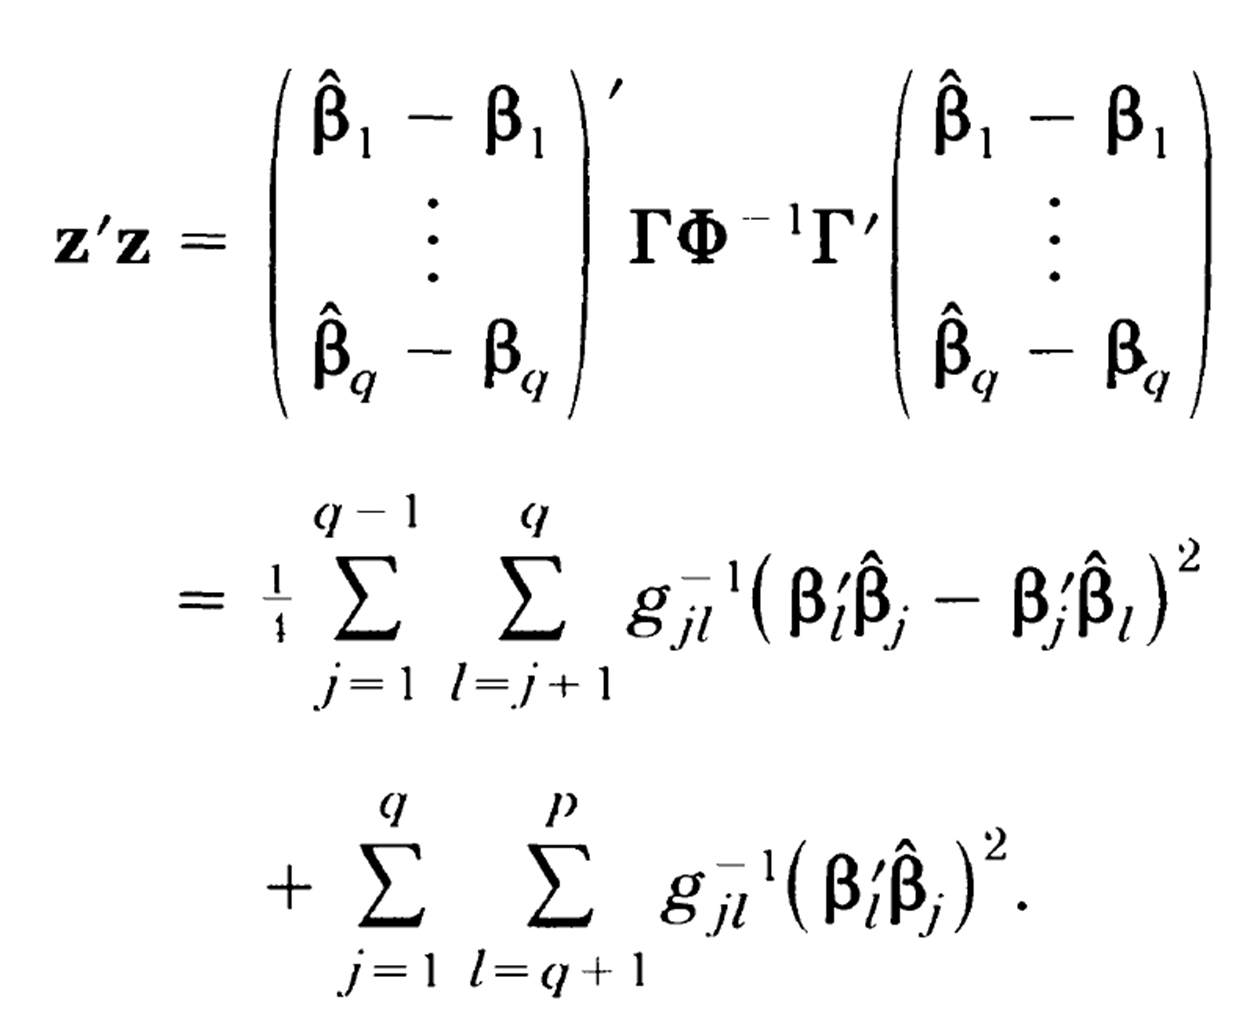
\includegraphics[width=0.5\linewidth]{image011.png}
	\end{figure}
	follows $\chi^2(t)$ distribution.
\end{frame}

%----------------------------------------------
\begin{frame}
	\frametitle{An asymptotic test for q hypothetical eigenvectors}
	This leads to the distribution of the test statistics for  $H_q: (\bm{\beta}_1,\ldots,\bm{\beta}_q) = (\bm{\beta}_1^0,\ldots,\bm{\beta}_q^0)$:
	\begin{figure}
		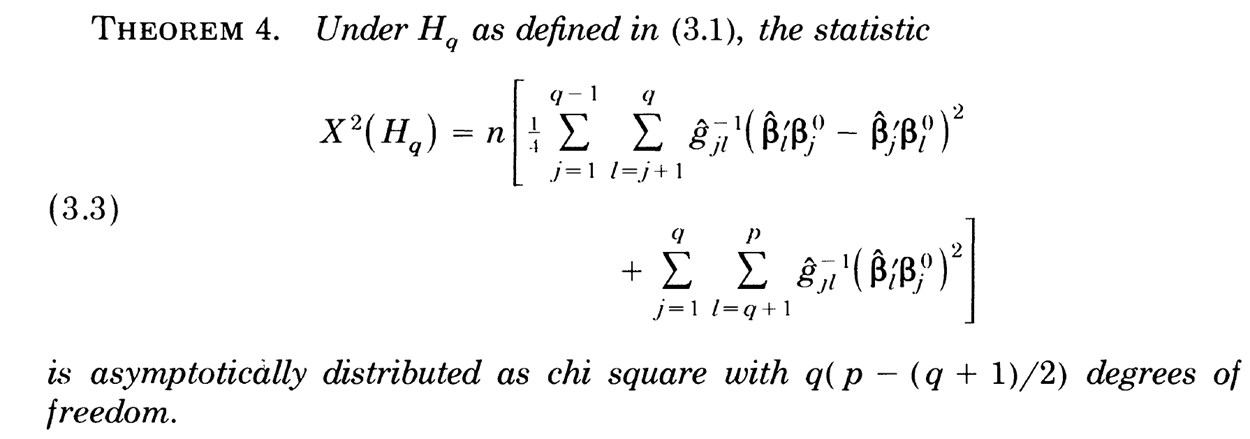
\includegraphics[width=.9\linewidth]{image012.png}
	\end{figure}
The paper also illustrated 2 special cases: (1) $q=1$ and (2) $q = p$.
\end{frame}

\section{inference for eigenvalues}

%----------------------------------------------
\begin{frame}
	\frametitle{Asymptotic inference for eigenvalues}
	Similar to regular PCA, we may need to discard CPC's with relatively small variances.\\
	Let $c_i=\sum_{j=1}^{q}\lambda_{ij}$, $d_i = tr\Sigma_i - c_i$, $f_i = d_i/tr\Sigma_i$ (relative contribution to trace) and $f_0$ be the pre-specified fraction. Then,
	\begin{figure}
		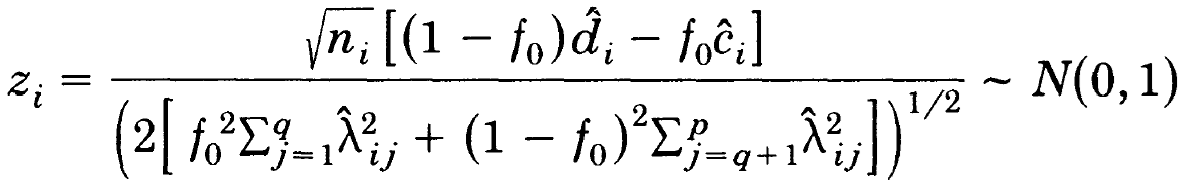
\includegraphics[width=.7\linewidth]{image013.png}
	\end{figure}
	when $f_i = f_0$ (null hypothesis).\\
	So for testing the $H_1$: all $f_i$ are less than or equal to $f_0$, we can just reject the hypothesis if 
	\begin{figure}
		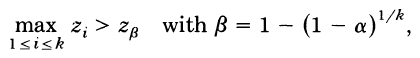
\includegraphics[width=.5\linewidth]{image014.png}
	\end{figure}
\end{frame}


%----------------------------------------------
\begin{frame}
	\frametitle{LRT for sphericity of p-q CPC's}
	In PCA, the motivation for testing equality of p-q characteristic roots stems from the model $\Sigma = \Psi + \sigma^2\bm{I}_p$, where $\Psi$ is p.s.d. of rank q.\\
	
	In CPCA, we can consider similar model for each group, i.e. $\Sigma_i = \Psi_i + \sigma_i^2\bm{I}_p$, with $\Psi_i$ be simultaneously diagonalizable and of rank q. This is equivalent as the following test (\textbf{hypothesis of partial sphericity}):
	$$H_S: \lambda_{i,q+1}=\ldots=\lambda_{ip}$$
	Putting $H_S: \lambda_{i,q+1}=\ldots=\lambda_{ip} = \lambda_i^*$, we get
	\begin{figure}
		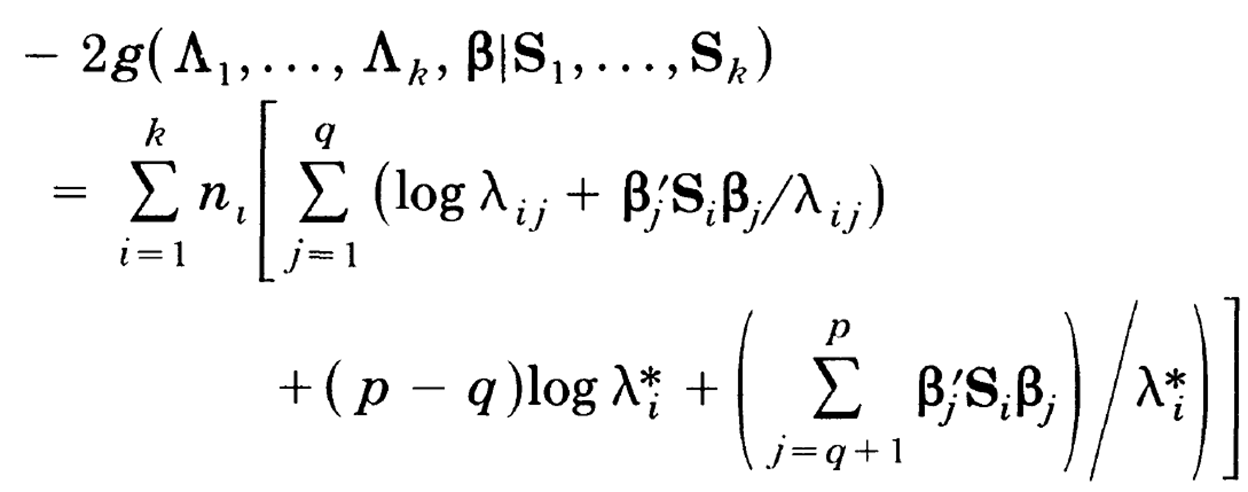
\includegraphics[width=.6\linewidth]{image015.png}
	\end{figure}
\end{frame}

%----------------------------------------------
\begin{frame}
	\frametitle{LRT for sphericity of p-q CPC's}
	After some algebra, we can get the LRT test statistic:
	\begin{figure}
		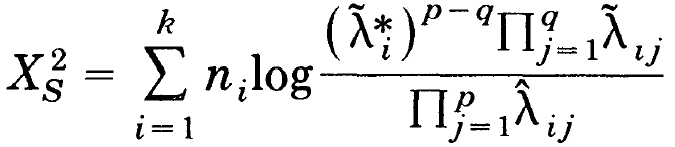
\includegraphics[width=.4\linewidth]{image017.png}
	\end{figure}
	The null distribution of $X_S^2$ is asymptotically $\chi^2((p-q-1)(p-q+2k)/2)$.
	The paper also provided the approximated statistic:
	\begin{figure}
		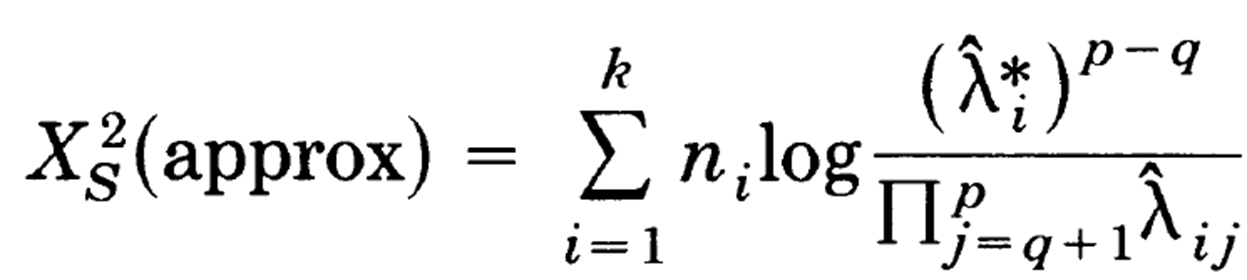
\includegraphics[width=.4\linewidth]{image018.png}
	\end{figure}
	But we need to be careful: since $X_S^2(approx)\geq X_S^2$, the approximate statistic can be used to accept $H_S$, but not necessarily to reject it.
\end{frame}


\section{Applications}
%----------------------------------------------
\begin{frame}
	\frametitle{Applications}
	Data: 2 groups (24 males and 24 females), with 3 features.\\
	We do log-transformation of data because of their relationship to allometry.The data and MLE's are shown in the table:
	\begin{figure}
		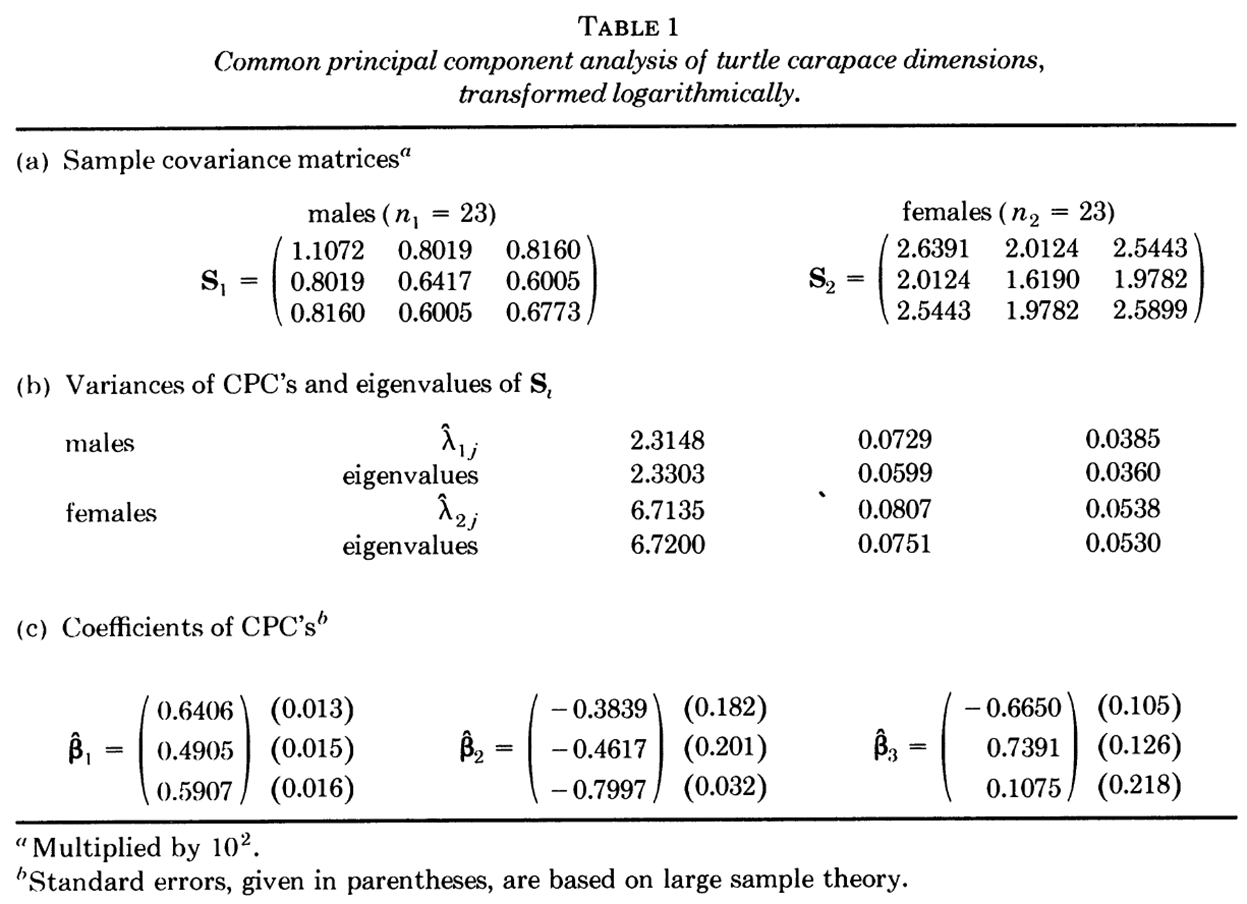
\includegraphics[width=.8\linewidth]{image019.png}
	\end{figure}
\end{frame}

%----------------------------------------------
\begin{frame}
	\frametitle{Applications}
	\textbf{Test 1}: if allometric growth is true, then the first PC of log-data should be $\bm{\beta}'_1 = (1,\ldots,1)/\sqrt{p}$. Therefore, the test is $H_0: \bm{\beta}_1 = \bm{\beta}^0_1 = (1,\ldots,1)'/\sqrt{3}$
	The test statistic $X^2(H_1) = 46.17$, which follows $\chi^2(2)$ under null. $\Rightarrow$  reject the null.
	
	\textbf{Test 2}: test $H_S:\lambda_{i2} = \lambda_{i3}$ for $i=1,2$ (simultaneous sphericity of the second and third CPC's).
	The resulting statistic is $X_S^2(approx) = 3.24$, which (approximately) follows $\chi^2(3)$ under the null. $\Rightarrow$ fail to reject.\\
	
	Taking into consideration the relative smallness of these 2 roots in both groups
	$\Rightarrow$
	\begin{itemize}
		\item 
		the 3 shell dimensions are distributed about a single principal axis ("size") and 2 minor axes.
		\item
		the main axis having the same orientation in space for both groups.
	\end{itemize}
	
	 
	 
	
	
	
	
	
	
	
	
	
\end{frame}
	
	
\end{document}